\section{Process' perspective}
\subsection{Our CI/CD pipeline}
To support agility we implemented a fully automated CI/CD pipeline \ref{fig:ci-quality-check} using GitHub Actions. This choice was made because of its seamless integration with GitHub and its free tier of 2,000 Linux runner minutes per month which met our operational requirements.

\subsubsection{Continuous Integration}

Every time a Pull Request (PR) is opened, a series of automated Continuous Integration(CI) workflows are triggered to enforce code quality, security, and compliance standards before merging to the main code base, see figure \ref{fig:ci-flow}.
\\
\begin{figure}[H]
    \centering
    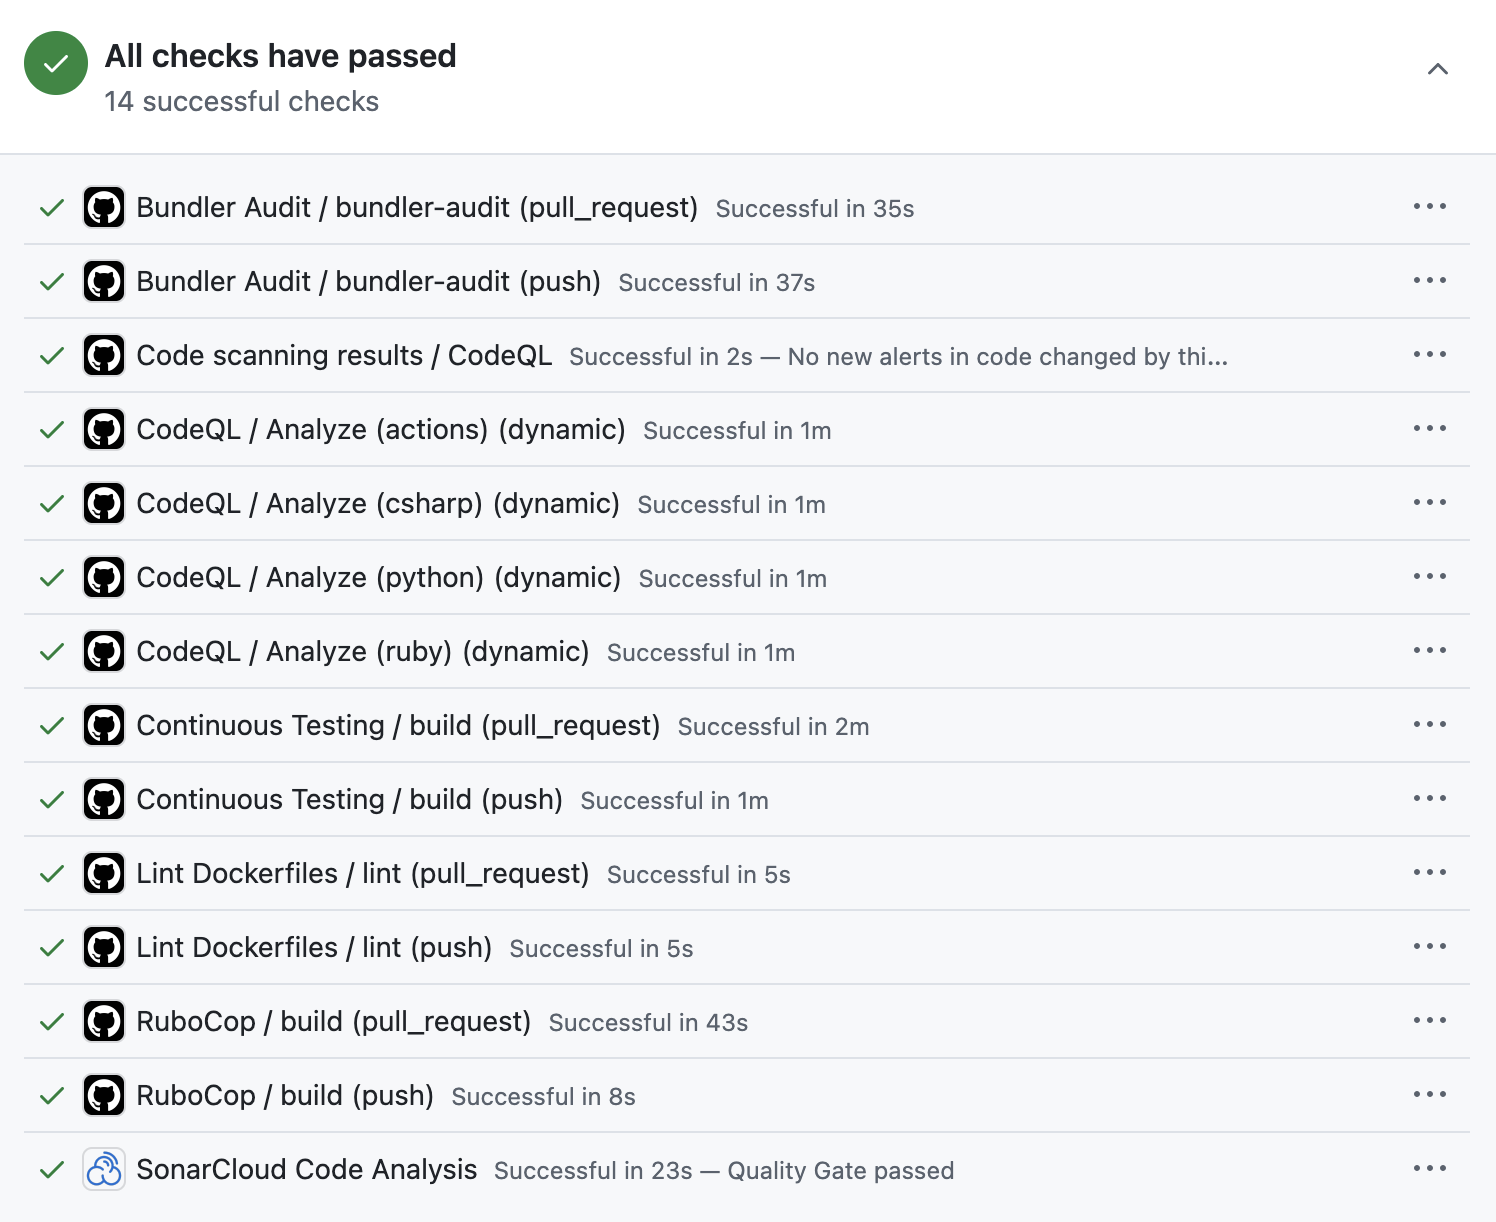
\includegraphics[width=0.7\linewidth]{images/ci pull-request quality check.png}
    \caption{Quality Check on Continuous Integration on each Pull Request}
    \label{fig:ci-quality-check}
\end{figure}

\noindent
All checks must pass before a PR can be merged, ensuring that only high-quality, secure code is integrated into the main branch.

\begin{figure}[H]
    \centering
    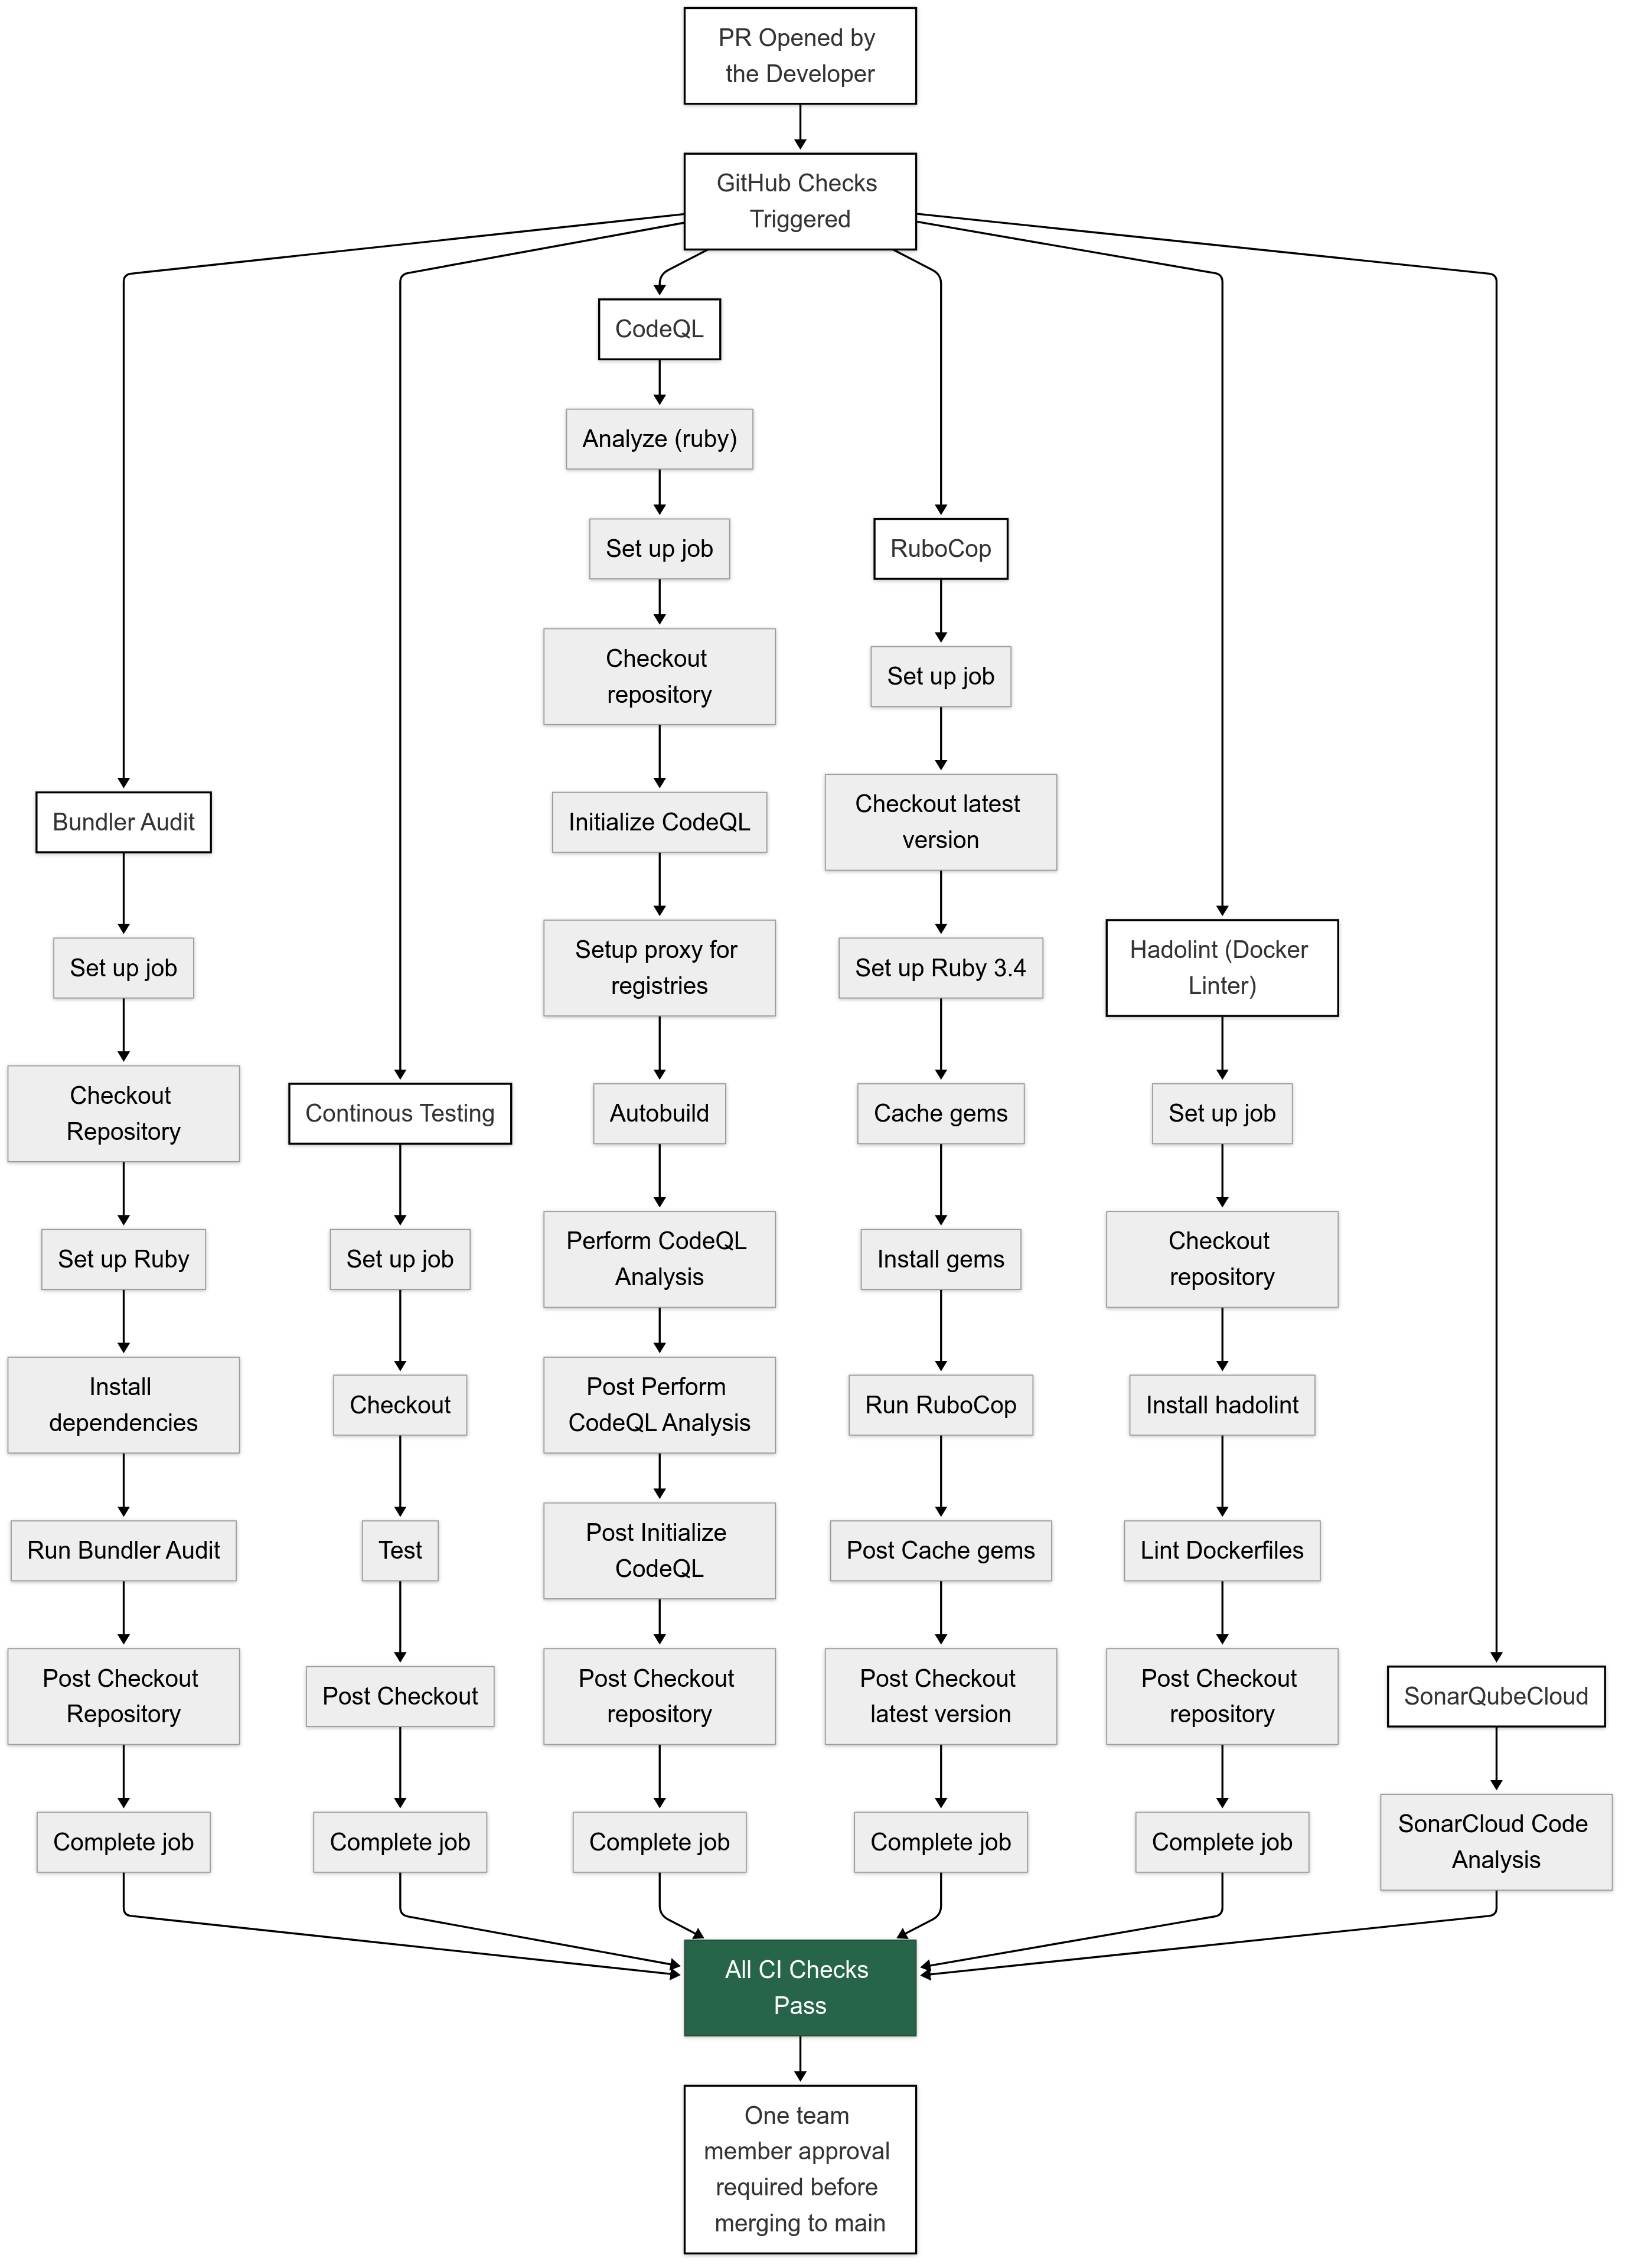
\includegraphics[width=0.75\linewidth]{images/CI pipeline.png}
    \caption{CI pipeline flow}
    \label{fig:ci-flow}
\end{figure}

\newpage
\subsubsection{Continuous Delivery}
Once a PR is merged into the \texttt{main} branch, two workflows \ref{fig:cd-flow} are triggered:
\\
\begin{enumerate}
  \item \textbf{Release Management} – A GitHub release is automatically created with a version tag, ensuring proper tracking and traceability of deployments.
  \item \textbf{Continuous Deployment} – Builds and pushes Docker images (\texttt{minitwitimage}, \texttt{flagtoolimage}) to Docker Hub, sets up SSH access, and deploys the new version of the application to the target server environment in DigitalOcean.
\end{enumerate}
%
After successful deployment, the application becomes immediately available in production.
\\

\begin{figure}[H]
    \centering
    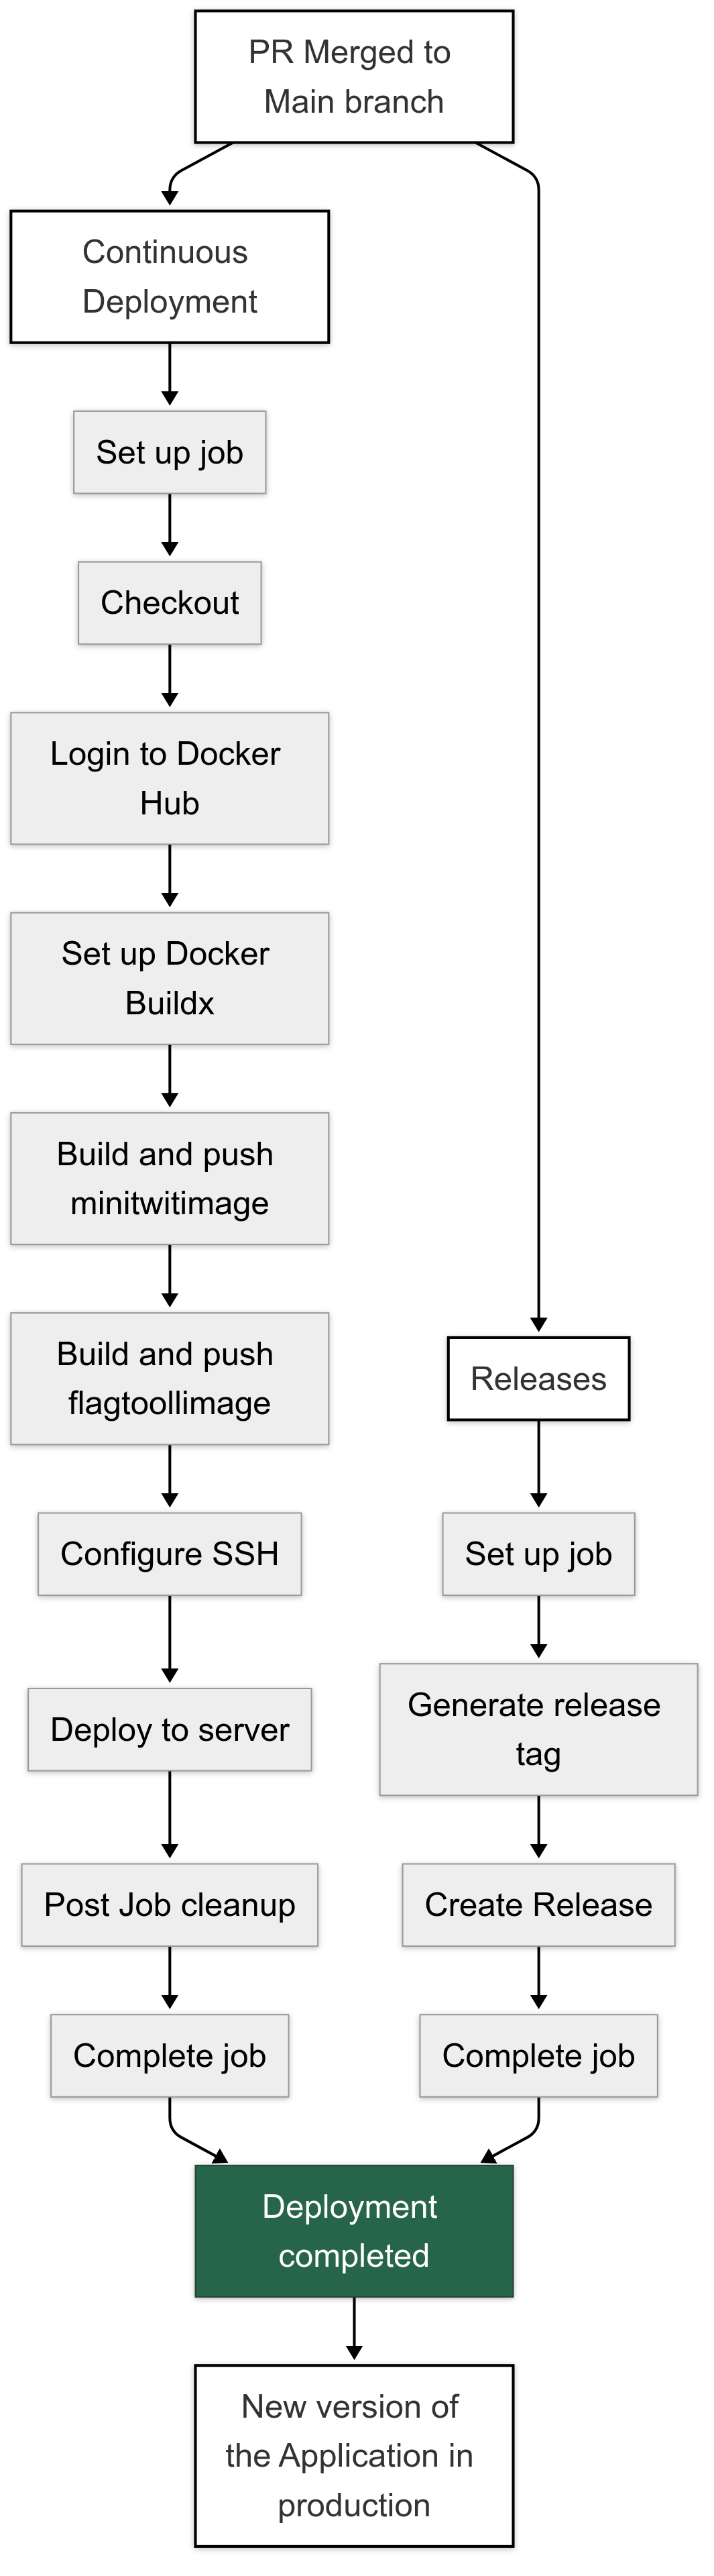
\includegraphics[width=0.25\linewidth]{images/CD pipeline.png}
    \caption{CD pipeline flow}
    \label{fig:cd-flow}
\end{figure}


%TC:ignore
\subsection{Monitoring}\label{section:monitoring}
%How do you monitor your systems and what precisely do you monitor? Chris
%TC:endignore

The monitoring of our application is done with Prometheus and Grafana \cite{grafana2025}. We chose these two systems due to them being industry standard, as well as the professors mentioning them as a possible option. Grafana and Prometheus are deployed in a Docker container situated on the manager node of our Docker swarm. 

Prometheus is configured to target our Minitwit application. Initially, we were also monitoring Prometheus itself, but after multiple weeks of our Prometheus container continuously mysteriously crashing, we decided to reduce the scraping. 

In addition to the default configuration for Grafana, we provide an admin user and password to our Dcompose file, preventing the resetting of credentials. Dashboards, datasources and alert rules are tracked in our Github repository and copied into the Grafana container upon creation. We discovered that this was needed shortly after implementing monitoring, when we realised that every deployment resets the dashboards.

Our dashboard (see Figure \ref{fig:grafana-dashboard}) keeps track of our server uptime and the average and maximum latency of requests, as well as requests per endpoint, status code, and ratio of return codes in percentage. Note that Figure \ref{fig:grafana-dashboard} was not captured when the simulator was running, but instead after it had stopped using the simulator script provided. Server uptime was the first metric we monitored, as we found it crucial to know whether our application was up or not. In addition to having a visualisation in our dashboard, we also set up an alert to send a message to our Discord server whenever Minitwit is down. When the simulator started, our application got a few errors due to our return codes not matching the ones expected by the simulator. That and us accidentally resetting our database multiple times made us want to track the return codes of our application, as well as the requests per endpoint, so that we could spot issues faster. Shortly after implementing monitoring, our application started slowing down in comparison to our classmates'. This led to the addition of the two latency endpoints, allowing us to keep track of the response time of our system. 
\\
\begin{figure}[H]
    \centering
    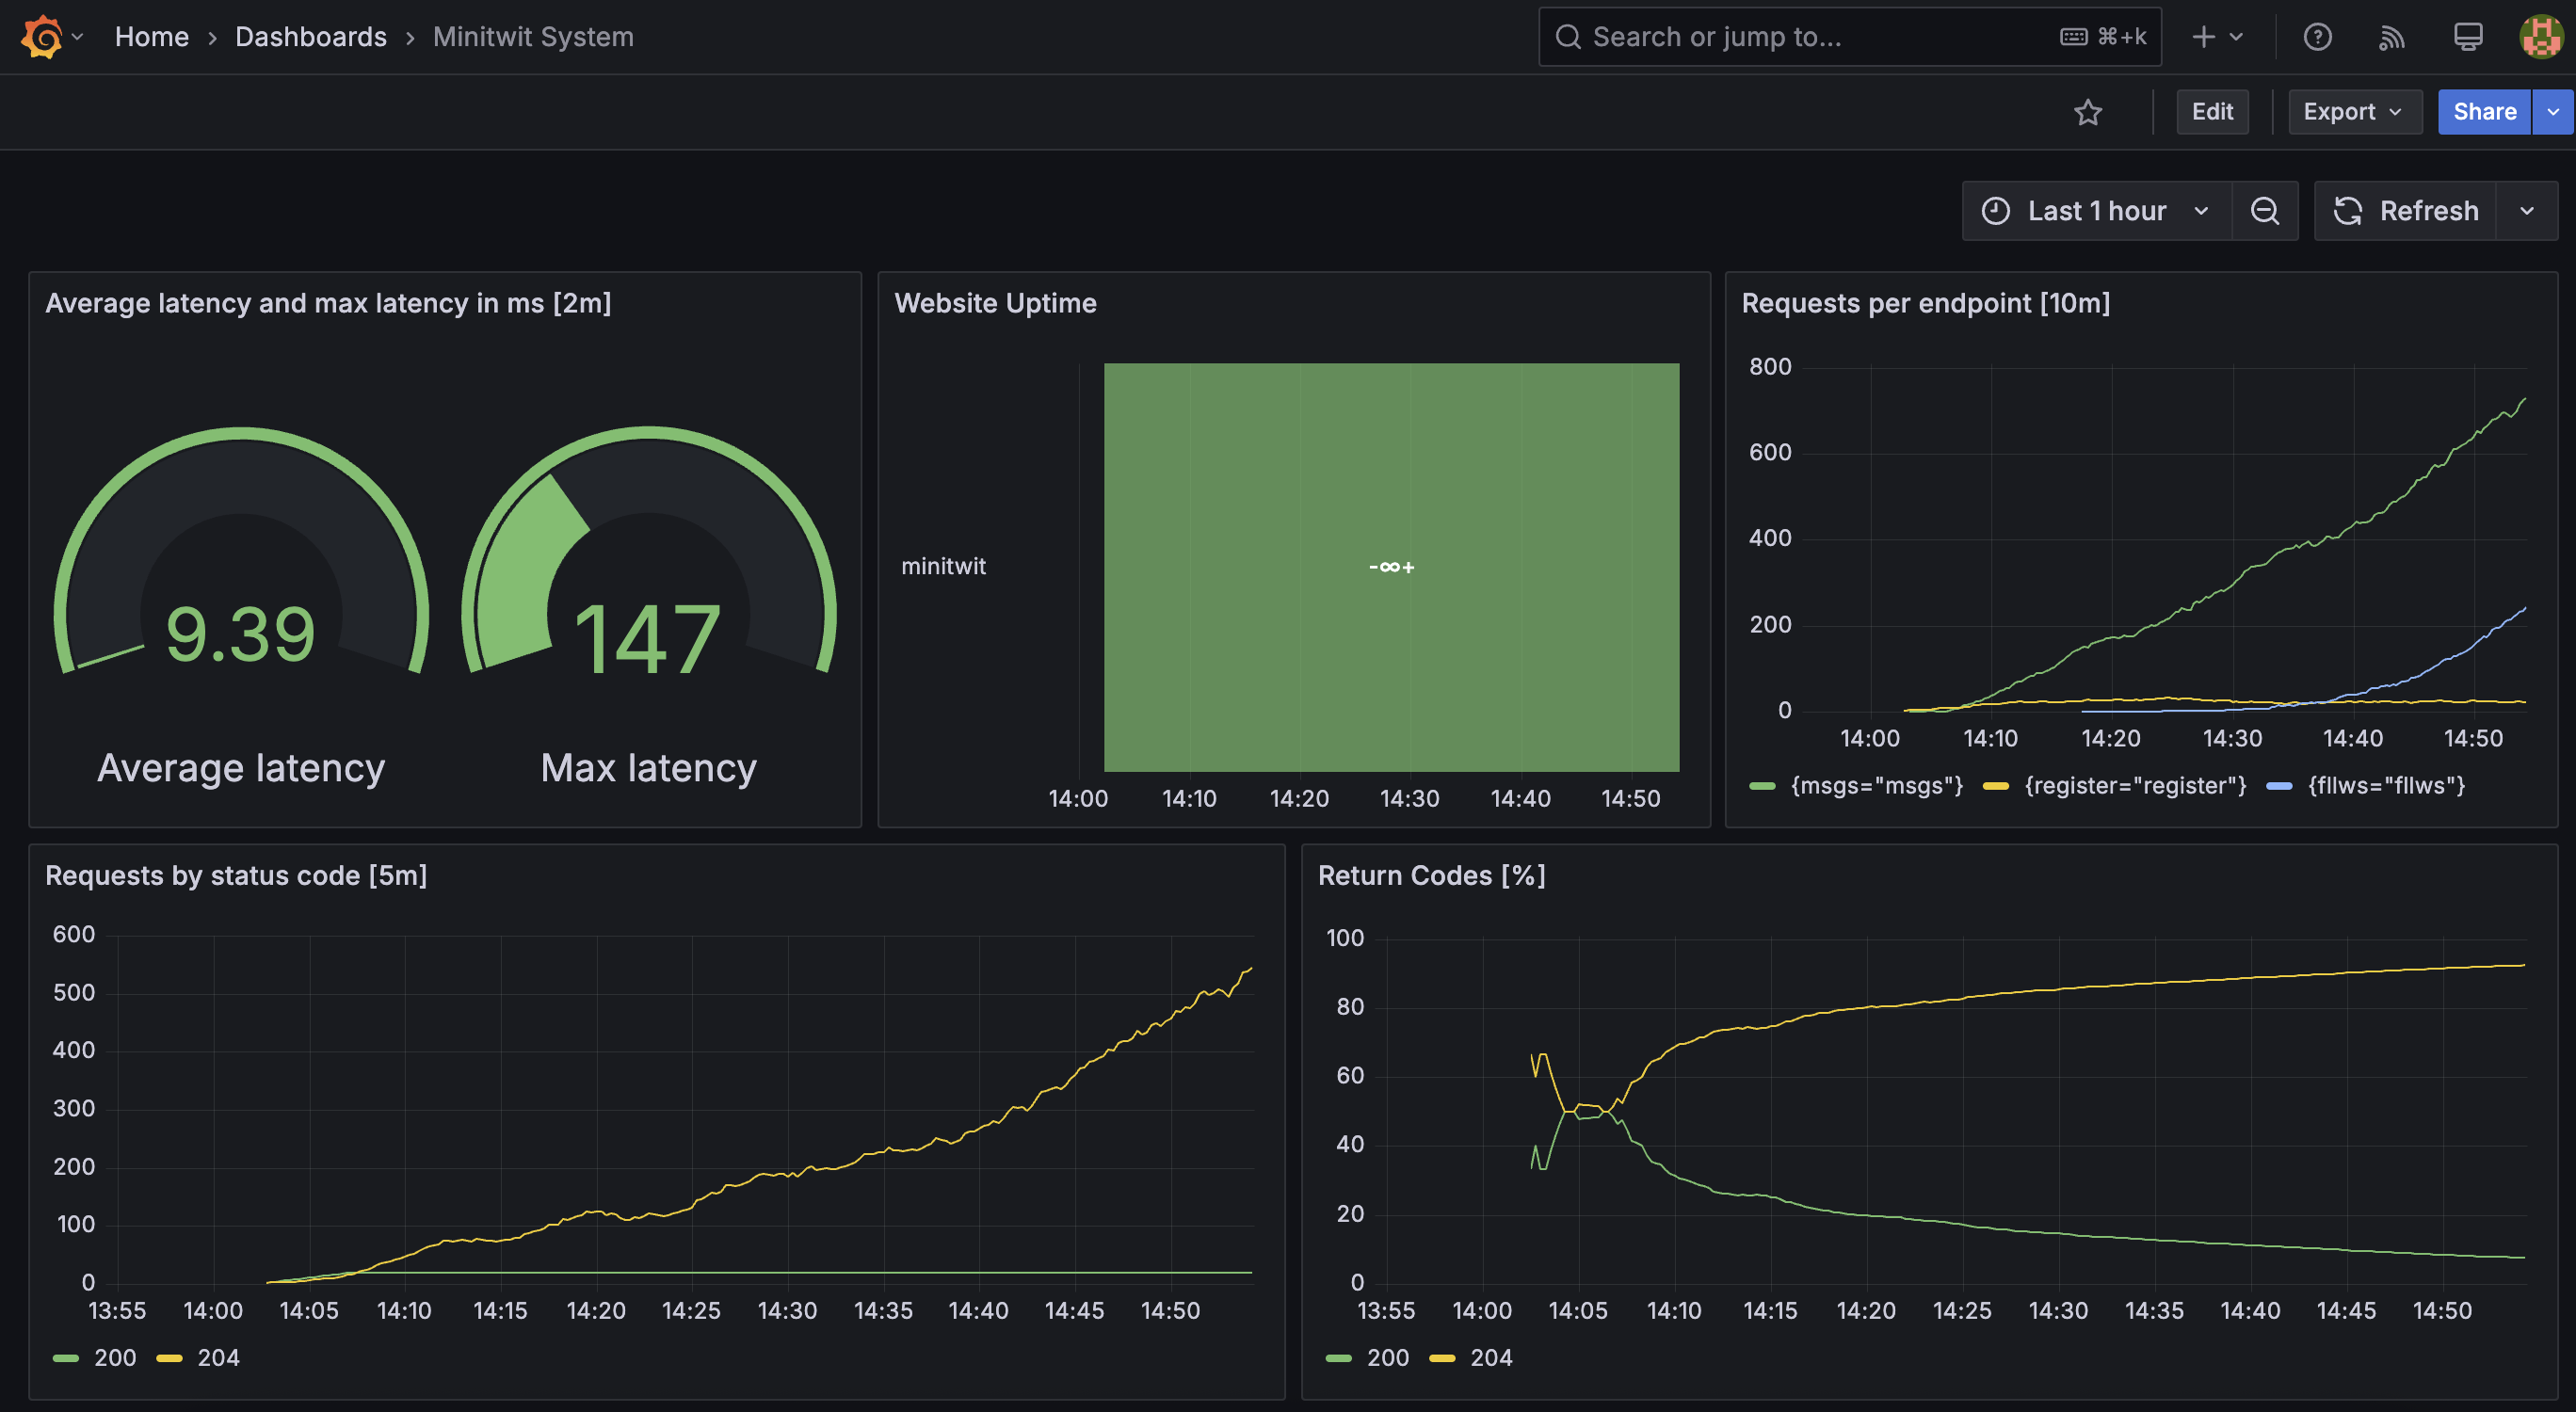
\includegraphics[width=0.95\linewidth]{images/grafana.png}
    \caption{Grafana dashboard after running the test simulator}
    \label{fig:grafana-dashboard}
\end{figure}
%
Our infrastructure is monitored using the built-in dashboard in DigitalOcean. It displays memory, CPU and disk usage.
\\
\subsection{Logging} \label{section:logging} %Daniel
The logging functionality in our system was implemented after the simulator ended using Ruby's native logging framework \cite{ruby_logger}. This built-in tool provides a simple yet flexible interface for outputting messages to standard output (STDOUT) or standard error (STDERR). Since our application runs within Docker containers, we leverage Docker's ability to capture STDOUT. This means all log messages are visible through the Docker logs, effectively mirroring what would appear in an interactive terminal session. This setup allows us to extract detailed runtime information from the application for monitoring and analysis.
\\
To collect and visualize logs from our Docker containers, we integrated Loki \cite{grafana_loki_docs} and Promtail \cite{grafana_promtail_docs} into our system. We chose these tools for log aggregation because they integrate seamlessly with our existing Prometheus and Grafana setup, allowing us to manage both metrics and logs within a unified Grafana interface. Promtail runs on every node and is responsible for forwarding Docker logs to Loki, as seen in Figure~\ref{fig:docker-swarm-services}.
\\
\begin{figure}[H]
    \centering
    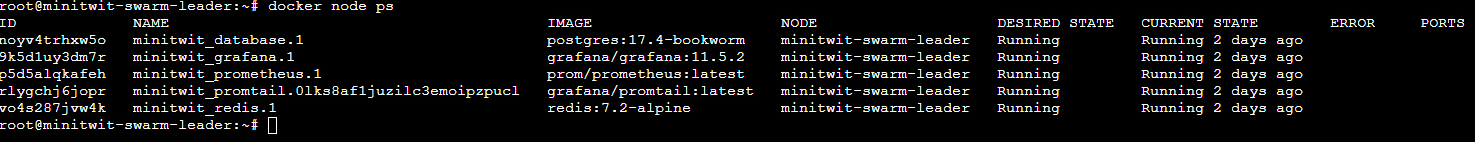
\includegraphics[width=\linewidth]{images/leader_docker_nodes.png}
    \caption{Overview of running services in the Docker Swarm leader node. The image shows the active containers for the Minitwit application, including services for the database, Grafana, Prometheus, Promtail, and Redis.}
    \label{fig:docker-swarm-services}
\end{figure}

Loki acts as the central log aggregation system. Unlike traditional logging systems that index the full log content, Loki is designed to index only the metadata with each log stream. This design choice, inspired by Prometheus, makes Loki more resource efficient and scalable. By configuring Loki as a data source in Grafana, we are able to query, filter, and visualize logs in real time.

\begin{figure}[H]
    \centering
    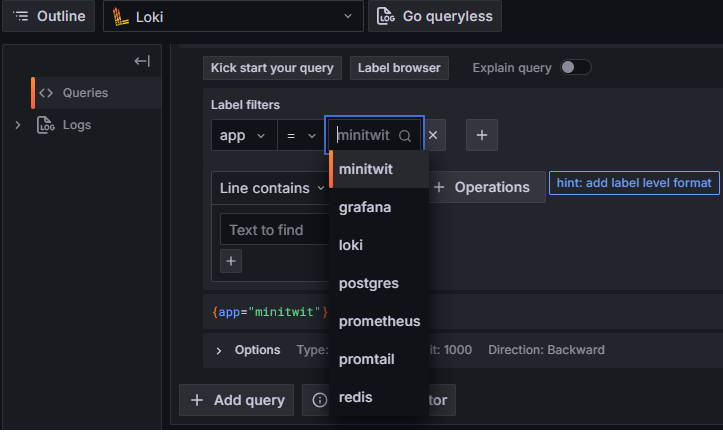
\includegraphics[width=0.5\linewidth]{images/Grafana_Explore.png}
    \caption{Grafana Explore interface showing log queries filtered by application label. This enables efficient selection and real-time inspection of logs from specific services.}
    \label{fig:grafana-explore}
\end{figure}

To illustrate the full pipeline from application log generation to visualization, the Ruby code below shows how we emit log messages at different severity levels:

\begin{lstlisting}[language=Ruby]
LOGGER = Logger.new($stdout)
LOGGER.info 'Home route hit'
LOGGER.warn 'Something might be off'
LOGGER.error 'Something went wrong'
\end{lstlisting}

These logs are captured by Docker, collected by Promtail and passed to Loki. As shown in Figure~\ref{fig:log-example}, they are then displayed in Grafana, where we can filter and view them in real time using the Explore interface.

\begin{figure}[H]
    \centering
    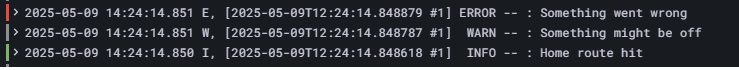
\includegraphics[width=\linewidth]{images/log_example.png}
    \caption{Logs generated using Ruby’s native logging framework\cite{ruby_logger}.}
    \label{fig:log-example}
\end{figure}


%TC:ignore
\subsection{Security} % Rakul :) <3 *.*
% Brief results of the security assessment and brief description of how did you harden the security of your system based on the analysis.
%TC:endignore

We performed a security assessment, identifying the following risk scenarios:

\begin{enumerate}
    \item Attacker performs SQL injection on web application to download user data.
    \item Attacker performs SQL injection on web application to delete user data.
    \item An attacker gets access to our environmental secrets and uses them to get access to our VM, DB, dashboards or Discord.
    \item An attacker exploits a vulnerability in a library.
    \item An attacker leaks passwords leading to unrecoverable business reputation.
    \item An attacker encrypts our DB leaving us unable to retrieve the DB.
    \item An attacker guesses or brute-forces weak passwords, gaining unauthorised access to users’ accounts.
\end{enumerate}

Each scenario was analysed, by discussing the impact and the probability of it. Finally, each scenario was mapped onto a risk matrix, see table \ref{tab:risk-matrix}.
Using the risk matrix, it was concluded that scenario 4 and 7 was the most relevant to address.
The impact of scenario 4 happening, really depended on what the attacker would exploit and what malicious things are done.
As the scenario was certain to happen, we hardened the security of our system by implementing the following:

\begin{enumerate}
    \item Enable Dependabot \cite{github_dependabot} to keep dependencies secure and up-to-date.
    \item Enable CodeQL analysis / Code Scanning \cite{github_codeql} to find security vulnerabilities and errors in our repository.
    \item Enable Secret Protection and Push protection \cite{github_secrets} which blocks commits that contain supported secrets.
\end{enumerate}

A proposed solution for scenario 7, was to setup a timeout after an amount of faulty tries, by placing a user in a lockdown mode with limited capabilities.
We also discussed setting up 2FA/MFA, however this was deemed out of scope.
For security measures that were already enforced, see appendix \ref{appendix:security}.

\begin{table}[H]
    \centering
    \begin{tabular}{c|c|c|c|c|c|c|}
        \cline{2-7}
        \multirow{6}{*}{\rotatebox[origin=c]{90}{\textbf{Impact} $\rightarrow$}} & \transparentcell{red}{0.4}{Catastrophic} & 3 & 2, 6 & & & 4 \\
        \cline{2-7}
        & \transparentcell{medium2}{0.4}{Critical} & & 1, 5 & & & 4 \\
        \cline{2-7}
        & \transparentcell{medium1}{0.4}{Marginal} & & & & & 4 \\
        \cline{2-7}
        & \transparentcell{low2}{0.4}{Negligible} & & & & 7 & 4 \\
        \cline{2-7}
        & \transparentcell{low1}{0.4}{Insignificant} & & & & & \\
        % Bottom axis label row without vertical bars
        \cline{2-7}
        & & \transparentcell{low1}{0.4}{Rare} & \transparentcell{low2}{0.4}{Unlikely} & \transparentcell{medium1}{0.4}{Possible} & \transparentcell{medium2}{0.4}{Likely} & \transparentcell{red}{0.4}{Certain} \\
        \cline{2-7}
        \multicolumn{7}{c}{\textbf{Probability} $\rightarrow$}
    \end{tabular}
    \caption{Risk matrix for security assesment.}
    \label{tab:risk-matrix}
\end{table}

\subsection{Scaling and Updates}\label{scaling} % Laurits

Our infrastructure leverages several technologies designed to ensure effective scaling and upgrade processes. Below, we explain our technology stack and strategies to optimize scaling capabilities and upgrade reliability.

\subsubsection{Hosting and Infrastructure with DigitalOcean}

We use DigitalOcean's virtual machines (VMs) for our hosting infrastructure due to their free credits through GitHub Education and the recommendation by the professors. DigitalOcean allows us to quickly spin up servers/droplets or scale existing resources vertically or horizontally.

\subsubsection{Terraform for Infrastructure Management}

Terraform was chosen for our Infrastructure as Code (IaC) solution. Using Terraform, we declaratively manage our infrastructure, ensuring consistency across deployments. Terraform simplifies the scaling process, as infrastructure changes are defined in code and applied systematically. It also streamlines upgrades and configuration changes by clearly maintaining state. Our Terraform state is securely stored in DigitalOcean Spaces, which ensures centralized, reliable, and collaborative management of infrastructure changes.

\subsubsection{Docker Swarm for Container Orchestration}\label{section:swarm-setup}

We use Docker Swarm for managing our containerized applications, which provides straightforward container orchestration suitable for our project scale. Docker Swarm allows easy horizontal scaling of services by simply increasing replica counts. For instance, our application is replicated three times, enabling load balancing and fault tolerance.

Docker Swarm supports zero-downtime updates through rolling updates, updating one replica at a time with start-first ordering, ensuring new containers start successfully before older ones are shut down. This guarantees uninterrupted service availability during upgrades.

\subsubsection{Overall Infrastructure}

The overall infrastructure is illustrated in Figure~\ref{fig:infrastructure}. Terraform is responsible for creating and maintaining a distributed Docker Swarm architecture with three node types:

\begin{enumerate}
  \item \textbf{Leader manager}
    \begin{enumerate}
      \item Maintains the cluster state and replicates updates to all other managers.
    \end{enumerate}

  \item \textbf{Managers}
    \begin{enumerate}
      \item Orchestrate container deployments and ensure the desired state is upheld across all worker nodes.
      \item Host our logging, monitoring, and database services.
      \item Participate in the Raft consensus protocol \cite{ongaro2014consensus} to keep the cluster state consistent in the event of leader failure.
    \end{enumerate}

  \item \textbf{Workers}
    \begin{enumerate}
      \item Run instances of our replicated Minitwit service.
    \end{enumerate}

\end{enumerate}

\begin{figure}[H]
    \centering
    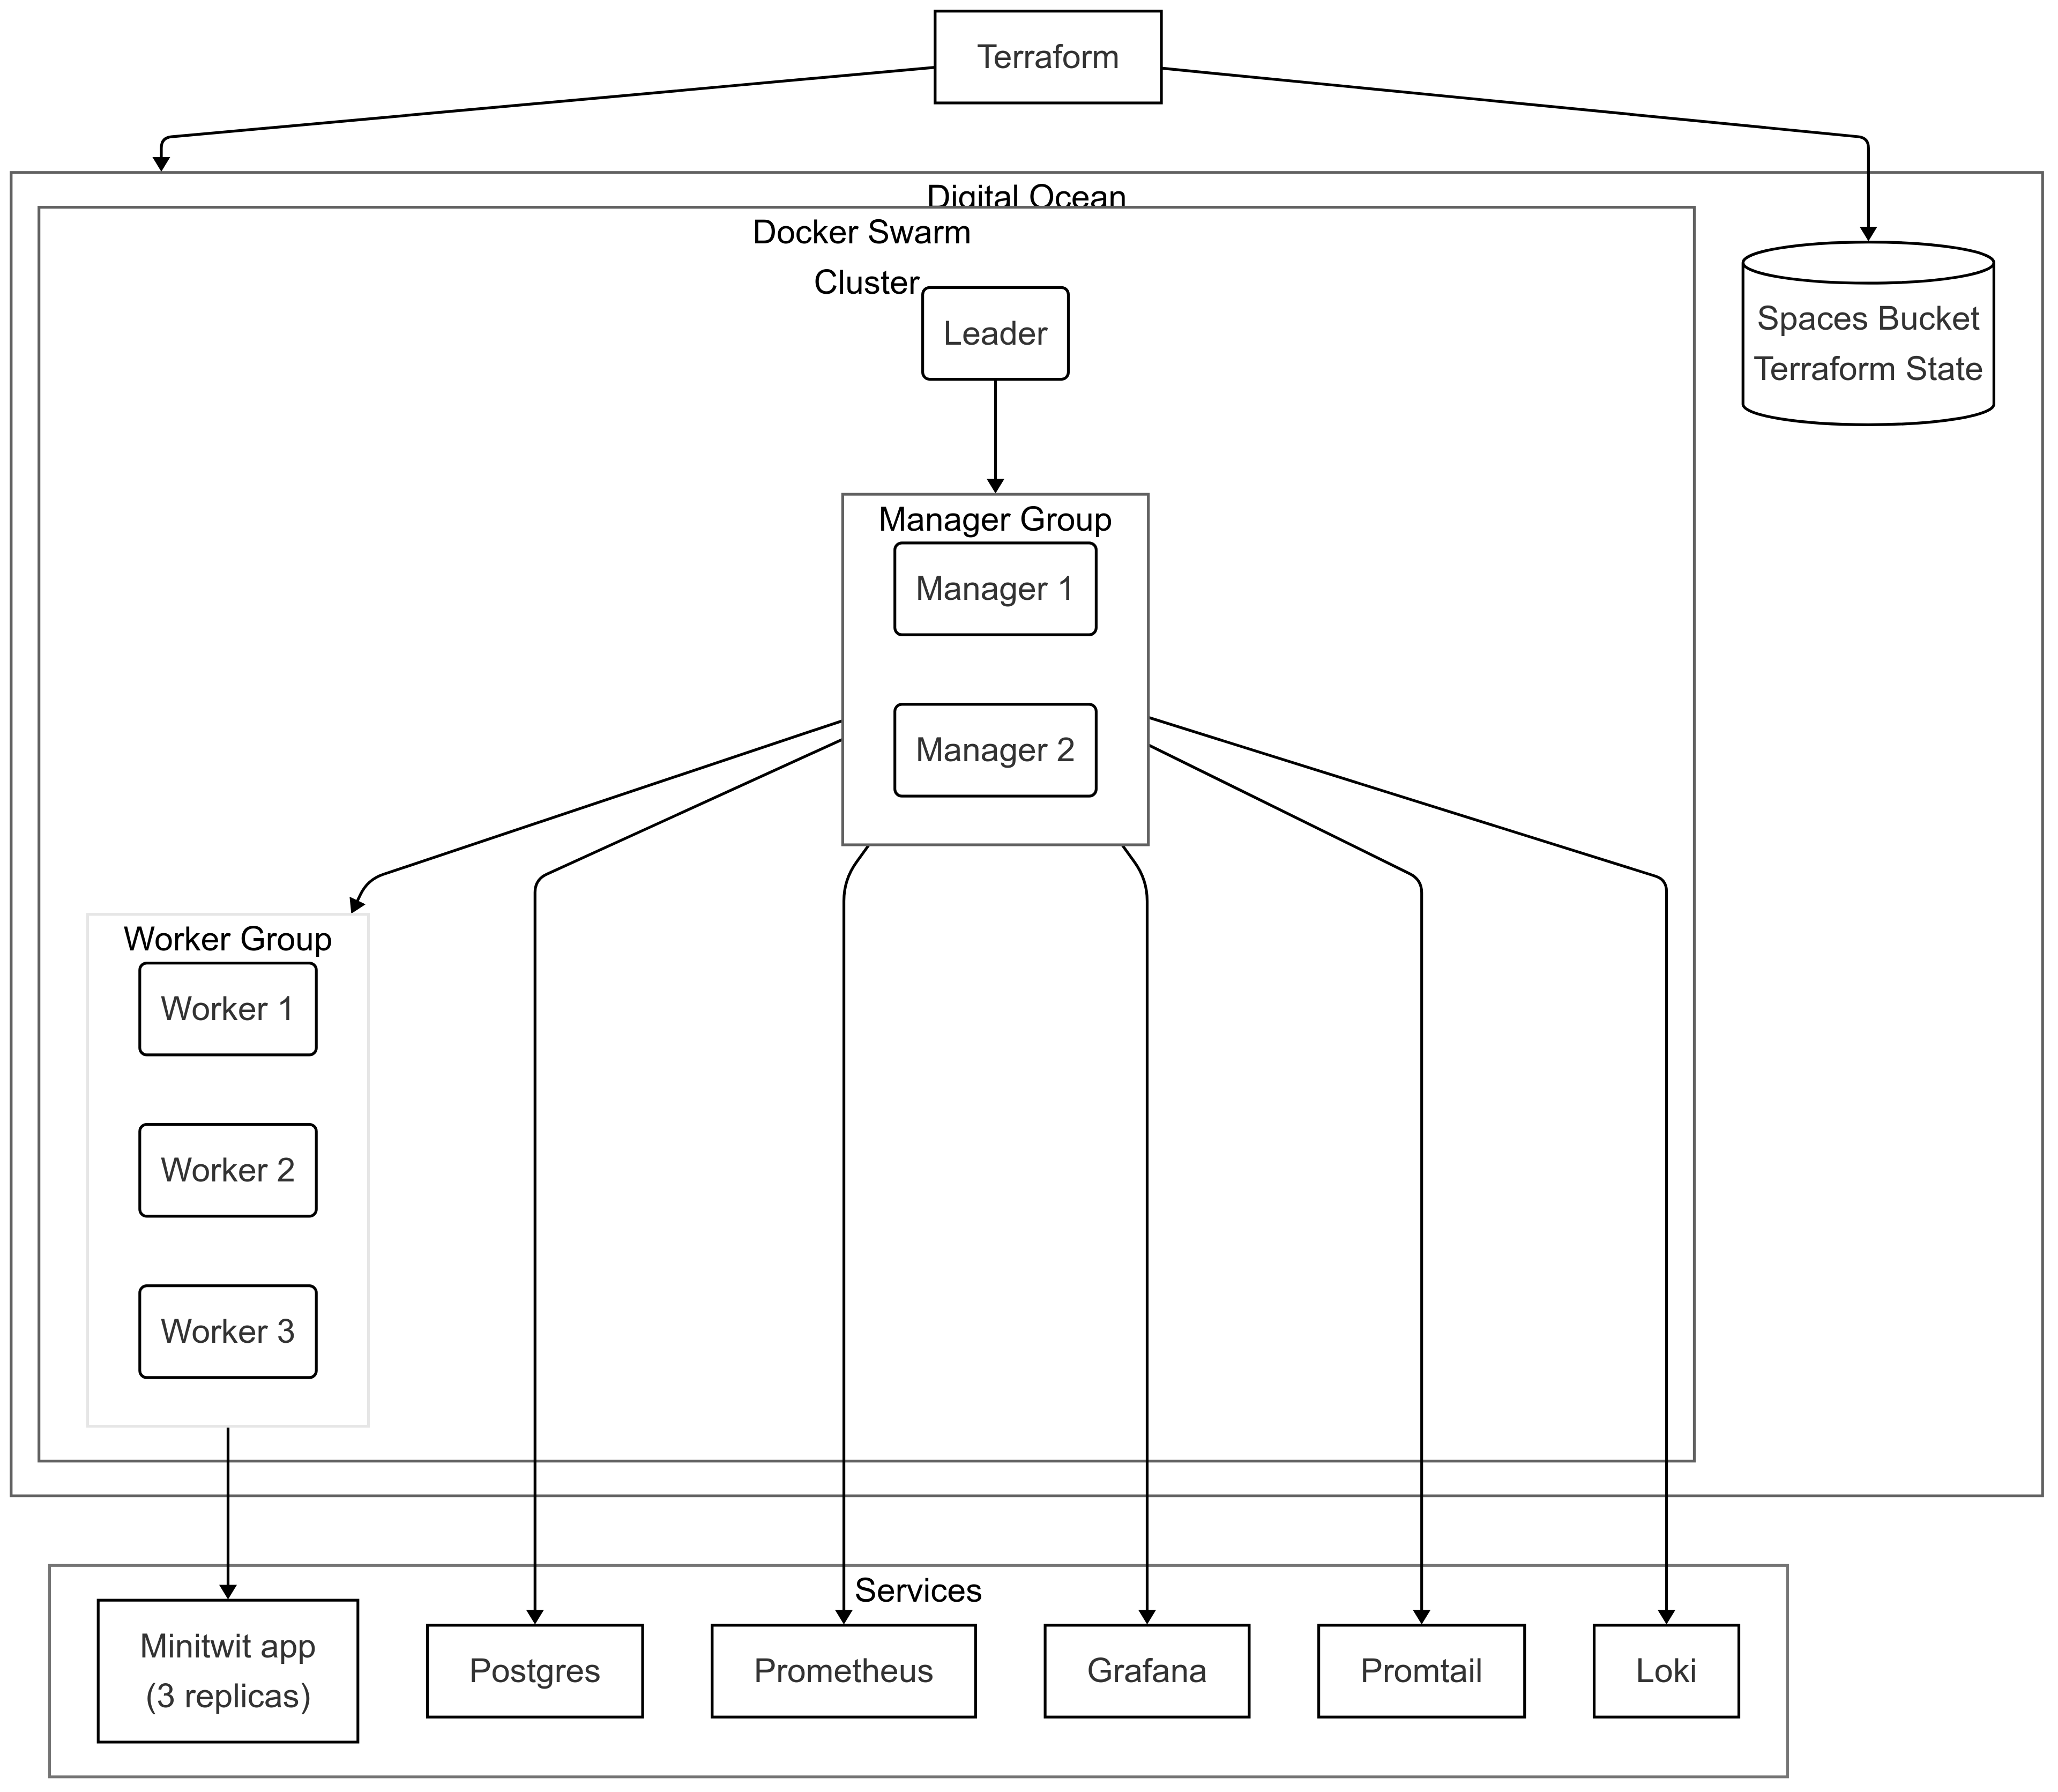
\includegraphics[width=1\linewidth]{images/diagram_infrastructure.png}
    \caption{High-Level Infrastructure Diagram}
    \label{fig:infrastructure}
\end{figure}



%TC:ignore
\subsection{Usage of AI-assistants} % Rakul :) <3 *.*
% In case you have used AI-assistants during your project briefly explain which system(s) you used during the project and reflect how it supported or hindered your process.
%TC:endignore

Throughout the project, we used generative AI, specifically ChatGPT, Claude and GitHub CoPilot, to assist us with programming tasks such as refactoring code. In the case of refactoring, using LLMs made the process faster but we still needed to do a lot of manual work since the solution proposed by the LLMs did not work out of the box. When setting up Docker Swarm, ChatGPT insisted it was easily done with a Vagrant file, but that turned out to be false and we realised hours later that a shell script was better suited.

